\chapter{Maxwell's equations and Conservation laws}
\section{Electrodynamics Before Maxwell}
Till now in electromagnetic theory we found out four equations which contribute to the foundation of Electromagnetic theory, and they are,
\begin{align*}{2}
\vec{\nabla} \cdot \vec{E}&=\frac{\rho}{\epsilon_{0}} \quad && \Rightarrow \text { Gauss' Law }  \\
\vec{\nabla} \cdot \vec{B}&=0 \quad && \Rightarrow \text { Gauss' Law for magnetism } \\
\vec{\nabla} \times \vec{E}&=-\frac{\partial \vec{B}}{\partial t} && \Rightarrow \text { Faraday's Law } \\
\vec{\nabla} \times \vec{B}&=\mu_{0}\left(\vec{J}\right) && \Rightarrow \text { Ampere's Law }
\end{align*}
There is a fatal inconsistency in these formulas. It has something to do with the old rule that divergence of curl is always zero $ (\nabla .(\nabla \times \mathbf{E})=0)$. If you apply the divergence to Faraday's law, everything works out: 
$$\nabla \cdot(\nabla \times \mathbf{E})=\nabla \cdot\left(-\frac{\partial \mathbf{B}}{\partial t}\right)=-\frac{\partial}{\partial t}(\nabla \cdot \mathbf{B})$$
The left side is zero because divergence of curl is zero; the right side is zero by virtue of Gauss law for magnetism. But when you do the same thing to Ampere's law, you get into trouble:$$\boldsymbol{\nabla} \cdot(\boldsymbol{\nabla} \times \mathbf{B})=\mu_{0}(\boldsymbol{\nabla} \cdot \mathbf{J})$$ The left side must be zero, but the right side, in general, is not. For steady currents, the divergence of $\mathbf{J}$ is zero, but evidently when we go beyond magnetostatics Ampère's law cannot be right.
\subsection{How Maxwell Fixed Ampere's Law}
Applying the continuity equation  and Gauss's law, in  Ampere's law the offending term can be rewritten as:
\begin{align*}
\nabla \cdot \mathbf{J}&=-\frac{\partial \rho}{\partial t}\\
&=-\frac{\partial}{\partial t}\left(\epsilon_{0} \nabla \cdot \mathbf{E}\right)\\&=-\nabla \cdot\left(\epsilon_{0} \frac{\partial \mathbf{E}}{\partial t}\right)
\end{align*}
If we were to combine $\epsilon_{0}(\partial \mathbf{E} / \partial t)$ with $\mathbf{J}$, in Ampère's law, it would be just right to kill off the extra divergence:$$\nabla \times \mathbf{B}=\mu_{0} \mathbf{J}+\mu_{0} \epsilon_{0} \frac{\partial \mathbf{E}}{\partial t}$$ Such a modification changes nothing, as far as magnetostatics is concerned: when $\mathbf{E}$ isconstant, we still have $\boldsymbol{\nabla} \times \mathbf{B}=\mu_{0} \mathbf{J}$.\\
Just as a changing magnetic field induces an electric field (Faraday's law), so \textbf{A changing electric field induces a magnetic field}.  Maxwell called his extra term the displacement current:

\hspace{5.10cm}\framebox{
	
	\parbox[t][2cm]{4cm}{
		
		\addvspace{0.2cm} \centering 
		Displacement Current
		$$\mathbf{J}_{d} \equiv \epsilon_{0} \frac{\partial \mathbf{E}}{\partial t}$$} 
}
\\\\ It's a misleading name, since $\epsilon_{0}(\partial \mathbf{E} / \partial t)$ has nothing to do with current, except that it adds to $\mathbf{J}$ in Ampère's law.
\subsection{Maxwell's Equations}
\begin{center}
	\framebox{
		\parbox[t][4.2cm]{3.5cm}{
			
			\addvspace{0.2cm} \centering
			
			\begin{align*}
			\begin{array}{lll}
			\textbf{(i)} & \nabla \cdot \mathbf{E}=\frac{1}{\epsilon_{0}} \rho&\text{(Gauss's law)} \\\\ \textbf{(ii)} & \nabla \cdot \mathbf{B}=0&\text{(No name.)}\\\\ \textbf{(iii)}& \boldsymbol{\nabla} \times \mathbf{E}=-\frac{\partial \mathbf{B}}{\partial t}&\text{(Faraday's law)}\\\\\textbf{(iv)}&\boldsymbol{\nabla} \times \mathbf{B}=\mu_{0} \mathbf{J}+\mu_{0} \epsilon_{0} \frac{\partial \mathbf{E}}{\partial t}&\text{(Ampère's law with
				Maxwell's correction)}
			\end{array}
			\end{align*}} }
\end{center}
Every phenomenon in electricity and magnetism can be derived from these equations. Many of our most important tools for various analyses come from the integral version of these equations, which are.
\begin{center}
	\framebox{
		\parbox[t][4.2cm]{3.5cm}{
			
			\addvspace{0.2cm} \centering
			
			\begin{align*}
			\begin{array}{lll}
			\textbf{(i)} & \iint_{S} \overrightarrow{\mathbf{E}} \cdot d \overrightarrow{\mathbf{A}}=\frac{Q}{\varepsilon_{0}} &\text{(Gauss's law)} \\\\ \textbf{(ii)} & \iint_{S} \overrightarrow{\mathbf{B}} \cdot d \overrightarrow{\mathbf{A}}=0&\text{(No name.)}\\\\ \textbf{(iii)}& \oint \overrightarrow{\mathbf{E}} \cdot d \overrightarrow{\mathbf{s}}=-\frac{d \mathbf{\phi_B}}{d t}&\text{(Faraday's law)}\\\\\textbf{(iv)}&\oint \overrightarrow{\mathbf{B}} \cdot d \overrightarrow{\mathbf{s}}=\mu_{0} I+\mu_{0} \varepsilon_{0} \frac{d \Phi_{E}}{d t}&\text{(Ampère's law with
				Maxwell's correction)}
			\end{array}
			\end{align*}} }
\end{center} 
Together with the force law,\ $\mathbf{F}=q(\mathbf{E}+\mathbf{v} \times \mathbf{B})$,\ they summarize the entire theoretical content of classical electrodynamics. Even the continuity equation,\ $\boldsymbol{\nabla} \cdot \mathbf{J}=-\frac{\partial \rho}{\partial t}$ \ which is the mathematical expression of conservation of charge, can be derived from Maxwell's equations by applying the divergence to Ampere's law.
\subsection{Maxwell's Equations In Free Space}
An extremely important limit of Maxwell's equations is found when there are no sources: $\rho=0, \vec{J}=0 .$ The equations become,
\begin{center}
	\framebox{
		\parbox[t][4.2cm]{3.5cm}{
			
			\addvspace{0.2cm} \centering
			
			\begin{align*}
			\begin{array}{lll}
			\textbf{(i)} & \nabla \cdot \mathbf{E}=0&\text{(Gauss's law)} \\\\ \textbf{(ii)} & \nabla \cdot \mathbf{B}=0&\text{(No name.)}\\\\ \textbf{(iii)}& \boldsymbol{\nabla} \times \mathbf{E}=-\frac{\partial \mathbf{B}}{\partial t}&\text{(Faraday's law)}\\\\\textbf{(iv)}&\boldsymbol{\nabla} \times \mathbf{B}=\mu_{0} \epsilon_{0} \frac{\partial \mathbf{E}}{\partial t}&\text{(Ampère's law with
				Maxwell's correction)}
			\end{array}
			\end{align*}} }
\end{center}
\subsection{Maxwell's Equations in Matter}
For inside polarized matter there will be accumulations of "bound" charge and current over which you exert no direct control. It would be nice to reformulate Maxwell's equations in such a way as to make explicit reference only to those sources we control directly: the "free" charges and currents. \\
We have already learned, from the static case, that an electric polarization $\mathbf{P}$ produces a bound charge density $$\rho_{b}=-\nabla \cdot \mathbf{P}$$ Likewise, a magnetic polarization (or "magnetization") $\mathbf{M}$ results in a bound current $$\mathbf{J}_{b}=\nabla \times \mathbf{\mathbf { M }}$$ There's just one new feature to consider in the nonstatic case: Any change in the electric polarization involves a flow of (bound) charge (call it $\mathbf{J}_{p}$), which must be included in the total current. For suppose we examine a tiny chunk of polarized material The polarization introduces a charge density $\sigma_{b}=P$ at one end and $-\sigma_{b}$ at the other. If $P$ now increases a bit, the charge on each end increases accordingly. \\giving a net current $$d I=\frac{\partial \sigma_{b}}{\partial t} d a_{\perp}=\frac{\partial P}{\partial t} d a_{\perp}$$
\begin{figure}[H]
	\begin{center}
		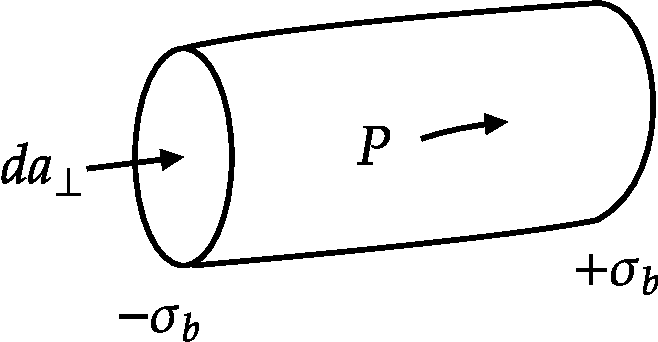
\includegraphics[width=4cm,height=2cm]{02-crop}
	\end{center}
\end{figure}
The current density, therefore, is $$\mathbf{J}_{p}=\frac{\partial \mathbf{P}}{\partial t}$$
This polarization current has nothing whatever to do with the bound current $\mathbf{J}_{b}$. The latter is associated with magnetization of the material and involves the spin and orbital motion of electrons; $\mathbf{J}_{p}$, by contrast, is the result of the linear motion of charge when the electric polarization changes. If $\mathbf{P}$ points to the right and is increasing, then each plus charge moves a bit to the right and each minus charge to the left; the cumulative effect is the polarization current $\mathbf{J}_{p}$\\\\
In fact, $\mathbf{J}_{p}$ is essential to account for the conservation of bound charge.\\
In view of all this, the total charge density can be separated into two parts: $$\rho=\rho_{f}+\rho_{b}=\rho_{f}-\boldsymbol{\nabla} \cdot \mathbf{P}$$ and the current density into three parts:
$$\mathbf{J}=\mathbf{J}_{f}+\mathbf{J}_{b}+\mathbf{J}_{p}=\mathbf{J}_{f}+\mathbf{\nabla} \times \mathbf{M}+\frac{\partial \mathbf{P}}{\partial t}$$ Gauss's law can now be written as $$\nabla \cdot \mathbf{E}=\frac{1}{\epsilon_{0}}\left(\rho_{f}-\nabla \cdot \mathbf{P}\right)$$ \text{or}$$\boldsymbol{\nabla} \cdot \mathbf{D}=\rho_{f}$$ where $\mathbf{D}$, as in the static case, is given by $$\mathbf{D} \equiv \epsilon_{0} \mathbf{E}+\mathbf{P}$$ Meanwhile, Ampère's law (with Maxwell's term) becomes $$\nabla \times \mathbf{B}=\mu_{0}\left(\mathbf{J}_{f}+\nabla \times \mathbf{M}+\frac{\partial \mathbf{P}}{\partial t}\right)+\mu_{0} \epsilon_{0} \frac{\partial \mathbf{E}}{\partial t}$$\text{or}$$\boldsymbol{\nabla} \times \mathbf{H}=\mathbf{J}_{f}+\frac{\partial \mathbf{D}}{\partial t}$$ where, as before,$$\mathbf{H} \equiv \frac{1}{\mu_{0}} \mathbf{B}-\mathbf{M}$$ Faraday's law and $\nabla \cdot \mathbf{B}=0$ are not affected by our separation of charge and current into free and bound parts, since they do not involve $\rho$ or $\mathbf{J}$. \\
In terms of free charges and currents, then, Maxwell's equations read\
\begin{center}
	\framebox{
		\parbox[t][2.5cm]{4cm}{
			
			\addvspace{0cm} \centering
			
			\begin{align*}
			\begin{array}{llll}
			\textbf{(i)} & \nabla \cdot \mathbf{D}=\rho_{f} &\textbf{(iii)} & \boldsymbol{\nabla} \times \mathbf{E}=-\frac{\partial \mathbf{B}}{\partial t},\\\\
			\textbf{(ii)}&\boldsymbol{\nabla} \cdot \mathbf{B}=0&\textbf{(iv)}& \boldsymbol{\nabla} \times \mathbf{H}=\mathbf{J}_{f}+\frac{\partial \mathbf{D}}{\partial t}
			\end{array}
			\end{align*}} }
\end{center}
for linear media
\begin{align*}
\begin{array}{lll}
\mathbf{P}=\epsilon_{0} \chi_{e} \mathbf{E} & and& \mathbf{M}=\chi_{m} \mathbf{H}\\\\
\mathbf{D}=\epsilon \mathbf{E}&and&\mathbf{H}=\frac{1}{\mu} \mathbf{B}
\end{array}
\end{align*}
where $\epsilon \equiv \epsilon_{0}\left(1+\chi_{e}\right)$ and $\mu \equiv \mu_{0}\left(1+\chi_{m}\right)$ D is called the electric "displacement"; that's why the second term in the Ampère/Maxwelf equation (iv) is called the displacement current,\\
In integral form Maxwell's equations in matter can be written as\\
\begin{align*}
\text{(i)}\hspace{0.5cm}\oint_{s}D\cdot da&=\theta_{fenc}\\
\text{(ii)}\hspace{0.5cm}\oint_{s}B\cdot da&=0\\
\text{(iii)}\hspace{0.5cm}\oint_{p}E\cdot dl&=\frac{-d}{dt}\int_{s} B\cdot da\\
\text{(iv)}\hspace{0.5cm}\oint_{p}H\cdot dl&=I_{end}+\frac{d}{dt}\int_{s} D\cdot da\\
\end{align*}
$P$ is the closed loop enclosing the surface $S$
\section{Boundary conditions}
In general the fields \textbf{E,B,D,} and \textbf{H} will be discontineous at a boundary between two different media or at surface that carries charge density $\sigma$ or current density \textbf{K}. The explicit form of the discontinities can be deduced from Maxwell's equations,in their integral form\\\\
$\left. \right. $\hspace{0.28cm} (i) $\oint_s \mathbf{D} \cdot d \mathbf{a}=Q_{f_{\mathrm{enc}}}$\\\\
$\left. \right. $\hspace{0.3cm}(ii) $\oint_s \mathbf{B} \cdot d \mathbf{a}=0$\\\\
$\left.\begin{array}{ll}\text { (iii) } \oint_l \mathbf{E} \cdot d \mathbf{l} & =-\frac{d}{d t} \int_s \mathbf{B} \cdot d \mathbf{a} \\ \\
\text { (iv) } \oint_l \mathbf{H} \cdot d \mathbf{l} & =I_{f_{\text {enc }}}+\frac{d}{d t} \int_s \mathbf{D} \cdot d \mathbf{a}\end{array}\right\} \begin{aligned}&\text { for any surface } s \\&\text { bounded by the } \\&\text { closed loop } l .\end{aligned}$\\\\
Applying (i) to a tiny, wafer-thin Gaussian pillbox extending just slightly into the material on either side of the boundary, we obtain \\
\begin{figure}[H]
	\centering
	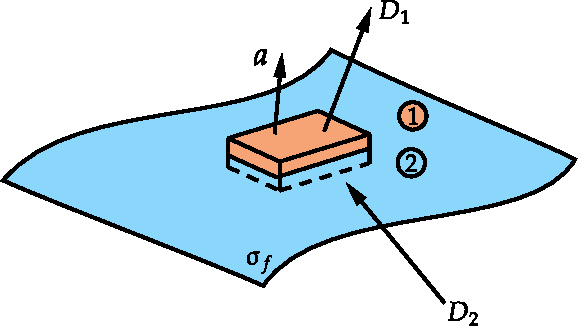
\includegraphics[height=4cm,width=7cm]{diagram-20220103(8)-crop}
	\caption{}
	\label{}
\end{figure}
$$\mathbf{D}_{1} \cdot \mathbf{a}-\mathbf{D}_{2} \cdot \mathbf{a}=\sigma_{f} a$$
Thus ,the component of D that is perperdicular to the interface is discontineous in the amount \\
$$D_{1}^{\perp}-D_{2}^{\perp}=\sigma_{f}$$
Identical reasoning,applied to equation(ii) yields\\
$$B_1^{\perp}-B_2^{\perp}=0$$
consider equation(iii) a very thin Amperian loop straddling the surface gives\\
\begin{figure}[H]
	\centering
	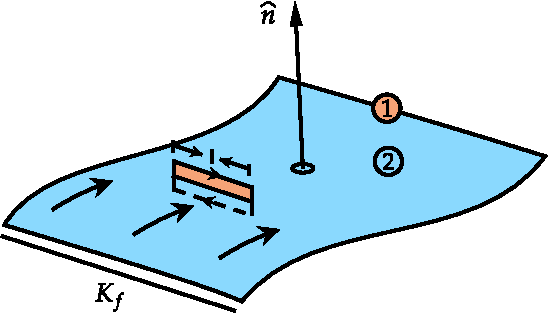
\includegraphics[height=4cm,width=7cm]{diagram-20220103(9)-crop}
	\caption{}
	\label{}
\end{figure}
$$E_1\cdot L-E_2\cdot L=-\frac{d}{dt} \int_{s} B\cdot da$$
But in the limit as the width of the loop goes to zero ,the flux vanishes.Therefore\\
$$E_1^{\parallel}-E_2^{\parallel}=0$$
That is the comonents of E parallel to the interface are contineous across the boundary.\\
equation (iv)  implies \\
$$H_1 \cdot L-H_2\cdot L=I_{f_{enc}}$$
Where $I_{f_{enc}}$ is the free current passing through the Amperian loop.No volume current density will contribute but a surface current can . In fact if $\hat{n}$ is a unit vector perpendicular to the interface so that $(\hat{n}\times L)$ is normal to the Amperian loop then,
$$I_{f_{enc}}=K_f \cdot (\hat{n}\times L)=(K_f\times \hat{n})\cdot L$$
And hence $$H_1^{\parallel}-H_2^{\parallel}=K_f\times \hat{n}$$
So the parallel components  H are discontinuous by an amount proportional to the free surface charge density.\\
In the case of linear media they can be expressed in terms of E and B alone 

\begin{enumerate}[label=(\roman*)]
	\item $\epsilon_{1} \mathbf{E}_{1}^{\perp}-\epsilon_{2} \mathbf{E}_{2}^{\perp}=\sigma_{f}$
	\item  $\mathbf{E}_{1}^{\|}-\mathbf{E}_{2}^{\|}=0$
	\item $\mathbf{B}_{1}^{\perp}-\mathbf{B}_{2}^{\perp}=0$
	\item $\frac{1}{\mu_{1}} \mathbf{B}_{1}^{\|}-\frac{1}{\mu_{2}} \mathbf{B}_{2}^{\|}=\mathbf{K}_{f} \times \hat{\mathbf{n}}$
\end{enumerate}

In particular, if there is no free charge or free current at the interface, then 
\begin{enumerate}[label=(\roman*)]
	\item $\epsilon_{1} \mathbf{E}_{1}^{\perp}-\epsilon_{2} \mathbf{E}_{2}^{\perp}=0$
	\item $\mathbf{E}_{1}^{\|}-\mathbf{E}_{2}^{\|}=0$
	\item $\mathbf{B}_{1}^{\perp}-\mathbf{B}_{2}^{\perp}=0$
	\item $\frac{1}{\mu_{1}} \mathbf{B}_{1}^{\|}-\frac{1}{\mu_{2}} \mathbf{B}_{2}^{\|}=0$
\end{enumerate}

\newpage
\begin{abox}
	Practise Set-1
\end{abox}
\begin{enumerate}
	\item The $x$ - and $z$-components of a static magnetic field in a region are $B_{x}=B_{0}\left(x^{2}-y^{2}\right)$ and $B_{z}=0$, respectively. Which of the following solutions for its $y$-component is consistent with the Maxwell equations?
	{\exyear{ NET/JRF-(JUNE-2016)}}
	\begin{tasks}(2)
		\task[\textbf{a.}]$B_{y}=B_{0} x y$
		\task[\textbf{b.}]$B_{y}=-2 B_{0} x y$
		\task[\textbf{c.}] $B_{y}=-B_{0}\left(x^{2}-y^{2}\right)$
		\task[\textbf{d.}]  $B_{y}=B_{0}\left(\frac{1}{3} x^{3}-x y^{2}\right)$
	\end{tasks}
	\item A current $i_{p}$ flows through the primary coil of a transformer. The graph of $i_{p}(t)$ as a function of time $t$ is shown in the figure below.\\
	\begin{figure}[H]
		\centering
		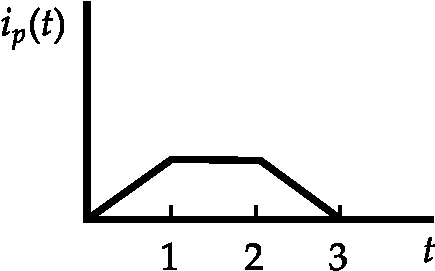
\includegraphics[height=3cm,width=4cm]{diagram-20211011(27)-crop}
	\end{figure}
	Which of the following graphs represents the current $i_{S}$ in the secondary coil?
	{\exyear{NET/JRF(JUNE-2014)}}
	\begin{tasks}(2)
		\task[\textbf{A.}] \begin{figure}[H]
			\centering
			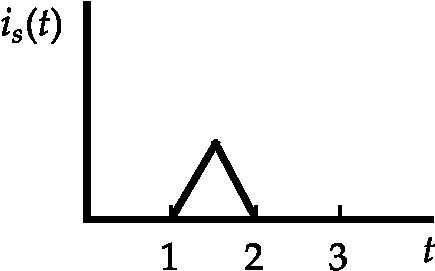
\includegraphics[height=3cm,width=4cm]{diagram-20211011(28)-crop}
		\end{figure}
		\task[\textbf{B.}] \begin{figure}[H]
			\centering
			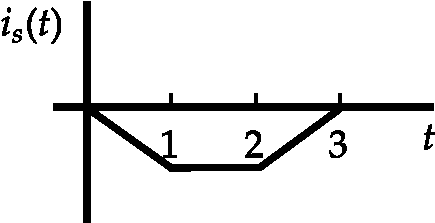
\includegraphics[height=3cm,width=4cm]{diagram-20211011(29)-crop}
		\end{figure}
		\task[\textbf{C.}] \begin{figure}[H]
			\centering
			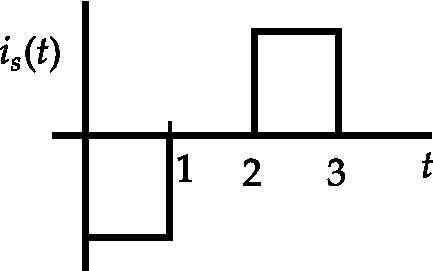
\includegraphics[height=3cm,width=4cm]{diagram-20211011(30)-crop}
		\end{figure}
		\task[\textbf{D.}] \begin{figure}[H]
			\centering
			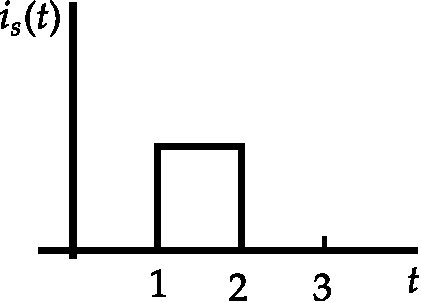
\includegraphics[height=3cm,width=4cm]{diagram-20211011(31)-crop}
		\end{figure}
	\end{tasks}
	\item A circular conducting wire loop is placed close to a solenoid as shown in the figure bellow. Also shown is the current through the solenoid as a function of solenoid as a function of time.\\
	\begin{figure}[H]
		\centering
		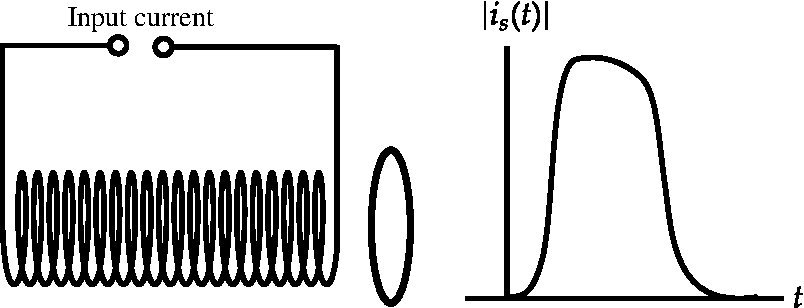
\includegraphics[height=3.5cm,width=9cm]{diagram-20211028(5)-crop}
	\end{figure}
	The magnitude $|i(t)|$ of the induced current in the wire loop, as a function of time $t$, is best represented as.
	{\exyear{NET/JRF(DEC-2019)}}
	\begin{tasks}(2)
		\task[\textbf{A.}] \begin{figure}[H]
			\centering
			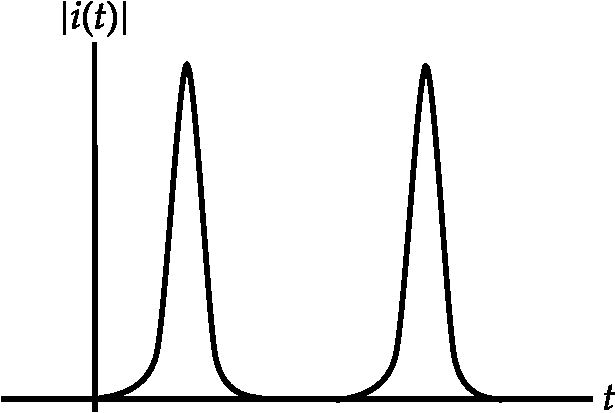
\includegraphics[height=3cm,width=5cm]{diagram-20211028(6)-crop}
		\end{figure}
		\task[\textbf{B.}] \begin{figure}[H]
			\centering
			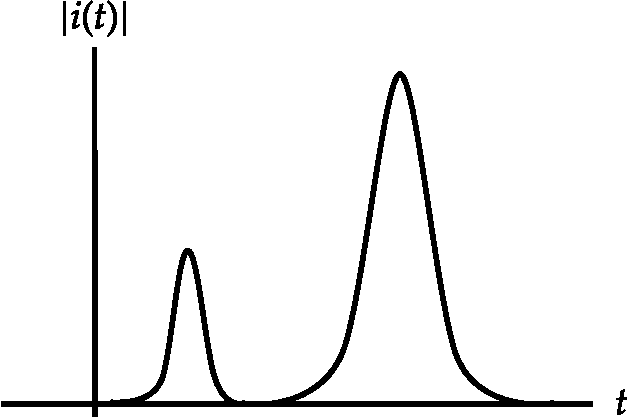
\includegraphics[height=3cm,width=5cm]{diagram-20211028(7)-crop}
		\end{figure}
		\task[\textbf{C.}] \begin{figure}[H]
			\centering
			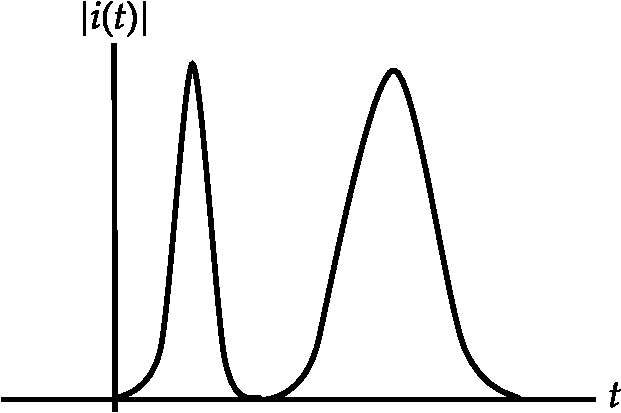
\includegraphics[height=3cm,width=5cm]{diagram-20211028(8)-crop}
		\end{figure}
		\task[\textbf{D.}] \begin{figure}[H]
			\centering
			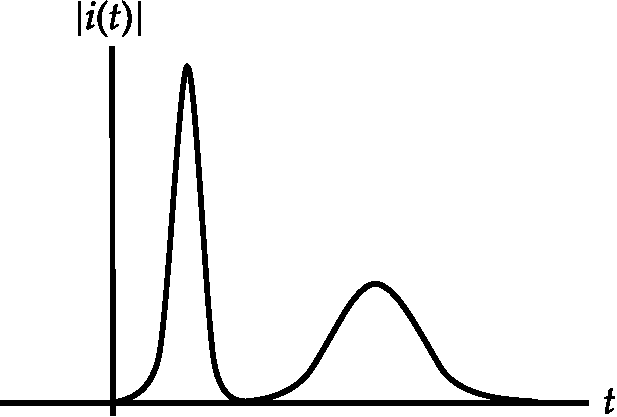
\includegraphics[height=3cm,width=5cm]{diagram-20211028(9)-crop}
		\end{figure}
	\end{tasks}
	\item A horizontal metal disc rotates about the vertical axis in a uniform magnetic field pointing up as shown in the figure. A circuit is made by connecting one end A of a resistor to the centre of the disc and the other end $B$ to its edge through a sliding contact. The current that flows through the resistor is
	{\exyear{NET/JRF(DEC-2013)}}
	\begin{figure}[H]
		\centering
		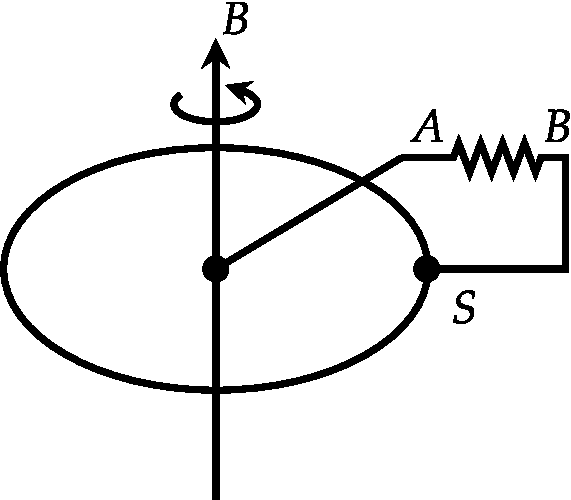
\includegraphics[height=4cm,width=5cm]{diagram-20211011(22)-crop}
	\end{figure}
	\begin{tasks}(4)
		\task[\textbf{A.}] Zero
		\task[\textbf{B.}] $D C$ from $A$ to $B$
		\task[\textbf{C.}] $D C$ from $B$ to $A$
		\task[\textbf{D.}] $A C$,
	\end{tasks}
	\item  A conducting circular disc of radius $r$ and resistivity $\rho$ rotates with an angular velocity $\omega$ in a magnetic field $B$ perpendicular to it. A voltmeter is connected as shown in the figure below. Assuming its internal resistance to be infinite, the reading on the voltmeter
	{\exyear{NET/JRF(DEC-2016)}}
	\begin{figure}[H]
		\centering
		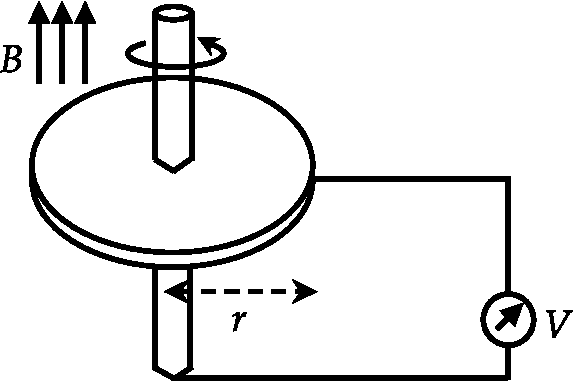
\includegraphics[height=3cm,width=5cm]{diagram-20211011(46)-crop}
	\end{figure}
	\begin{tasks}(1)
		\task[\textbf{A.}] Depends on $\omega, B, r$ and $\rho$
		\task[\textbf{B.}] Depends on $\omega, B$ and $r$ but not on $\rho$
		\task[\textbf{C.}]  Is zero because the flux through the loop is not changing
		\task[\textbf{D.}] Is zero because a current the flows in the direction of $B$
	\end{tasks}	
	\item A uniform magnetic field in the positive $z$-direction passes through a circular wire loop of radius $1 \mathrm{~cm}$ and resistance $1 \Omega$ lying in the $x y$-plane. The field strength is reduced from 10 tesla to 9 tesla in $1 s$. The charge transferred across any point in the wire is approximately
	{\exyear{ NET/JRF-(JUNE-2015)	}}
	\begin{tasks}(2)
		\task[\textbf{a.}] $3.1 \times 10^{-4}$ coulomb
		\task[\textbf{b.}]$3.4 \times 10^{-4}$ coulomb
		\task[\textbf{c.}]$4.2 \times 10^{-4}$ coulomb
		\task[\textbf{d.}] $5.2 \times 10^{-4}$ coulomb
	\end{tasks}	
	\item A magnetic field $B$ is $B \hat{z}$ in the region $x>0$ and zero elsewhere. A rectangular loop, in the $x y$-plane, of sides $l$ (along the $x$-direction) and $h$ (along the $y$-direction) is inserted into the $x>0$ region from the $x<0$ region at constant velocity $v=v \hat{x}$. Which of the following values of $l$ and $h$ will generate the largest EMF?
	{\exyear{ NET/JRF-(JUNE-2016)	}}
	\begin{tasks}(2)
		\task[\textbf{a.}] $l=8, h=3$
		\task[\textbf{b.}]$l=4, h=6$
		\task[\textbf{c.}]$l=6, h=4$
		\task[\textbf{d.}]  $l=12, h=2$
	\end{tasks}	
	\item Consider a solenoid of radius $R$ with $n$ turns per unit length, in which a time dependent current $I=I_{0} \sin \omega t$ (where $\omega R / c<<1$ ) flows. The magnitude of the electric field at a perpendicular distance $r<R$ from the axis of symmetry of the solenoid, is
	{\exyear{NET/JRF-(DEC-2011)	}}
	\begin{tasks}(2)
		\task[\textbf{a.}]0
		\task[\textbf{b.}]$\frac{1}{2 r} \omega \mu_{0} n I_{0} R^{2} \cos \omega t$
		\task[\textbf{c.}]$\frac{1}{2} \omega \mu_{0} n I_{0} r \sin \omega t$
		\task[\textbf{d.}]  $\frac{1}{2} \omega \mu_{0} n I_{0} r \cos \omega t$
	\end{tasks}	
	\item A parallel plate capacitor is formed by two circular conducting plates of radius a separated by a distance $d$, where $d \ll a$. It is being slowly charged by a current that is nearly constant. At an instant when the current is $I$, the magnetic induction between the plates at a distance $\frac{a}{2}$ from the centre of the plate, is
	{\exyear{ NET/JRF-(DEC-2016)}}	
	\begin{tasks}(2)
		\task[\textbf{a.}]$\frac{\mu_{0} I}{\pi a}$
		\task[\textbf{b.}]$\frac{\mu_{0} I}{2 \pi a}$
		\task[\textbf{c.}]$\frac{\mu_{0} I}{a}$
		\task[\textbf{d.}]  $\frac{\mu_{0} I}{4 \pi a}$
	\end{tasks}	
	\item Suppose the $y z$-plane forms a chargeless boundary between two media of permittivities $\epsilon_{\text {left }}$ and $\epsilon_{\text {right }}$ where $\epsilon_{\text {left }}: \epsilon_{\text {right }}=1: 2$, if the uniform electric field on the left is $\vec{E}_{\text {left }}=c(\hat{i}+\hat{j}+\hat{k})$ (where $c$ is a constant), then the electric field on the right $\vec{E}_{\text {right }}$ is
	{\exyear{NET/JRF(JUNE-2015)}}
	\begin{tasks}(4)
		\task[\textbf{A.}]  $c(2 \hat{i}+\hat{j}+\hat{k})$
		\task[\textbf{B.}] $c(\hat{i}+2 \hat{j}+2 \hat{k})$
		\task[\textbf{C.}] $c\left(\frac{1}{2} \hat{i}+\hat{j}+\hat{k}\right)$
		\task[\textbf{D.}] $c\left(\hat{i}+\frac{1}{2} \hat{j}+\frac{1}{2} \hat{k}\right)$
	\end{tasks}
	\item  The half space region $x>0$ and $x<0$ are filled with dielectric media of dielectric constants $\varepsilon_{1}$ and $\varepsilon_{2}$ respectively. There is a uniform electric field in each part. In the right half, the electric field makes an angle $\theta_{1}$ to the interface. The corresponding angle $\theta_{2}$ in the left half satisfies
	{{\exyear{NET/JRF(JUNE-2016)}}}
	\begin{figure}[H]
		\centering
		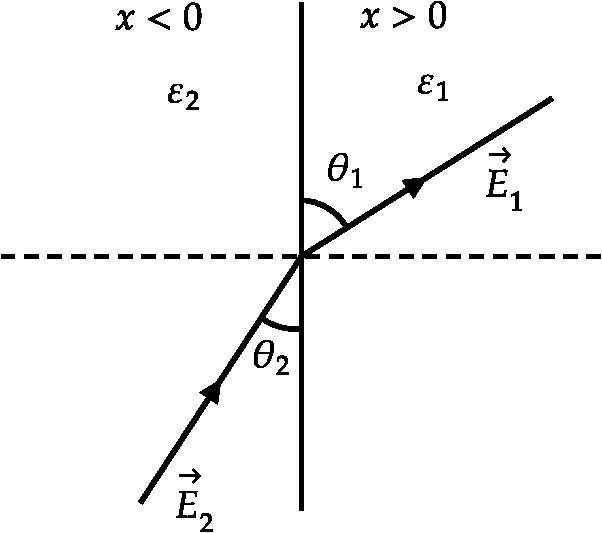
\includegraphics[height=4cm,width=5cm]{diagram-20211011(41)-crop}
	\end{figure}
	\begin{tasks}(2)
		\task[\textbf{A.}] $\varepsilon_{1} \sin \theta_{2}=\varepsilon_{2} \sin \theta_{1}$
		\task[\textbf{B.}] $\varepsilon_{1} \tan \theta_{2}=\varepsilon_{2} \tan \theta_{1}$
		\task[\textbf{C.}] $\varepsilon_{1} \tan \theta_{1}=\varepsilon_{2} \tan \theta_{2}$
		\task[\textbf{D.}] $\varepsilon_{1} \sin \theta_{1}=\varepsilon_{2} \sin \theta_{2}$
	\end{tasks}
	\item Which of the following is not a correct boundary condition at an interface between two homogeneous dielectric media? (In the following $\hat{n}$is a unit vector normal to the  interface, $\sigma$ and $\vec{j}_s$, are the surface charge and current densities, respectively.)
	{\exyear{NET/JRF(JUNE-2019)}}
	\begin{tasks}(2)
		\task[\textbf{A.}] $\hat{n} \times\left(\vec{D}_{1}-\vec{D}_{2}\right)=0$
		\task[\textbf{B.}] $\hat{n} \times\left(\vec{H}_{1}-\vec{H}_{2}\right)=\vec{j}_{s}$
		\task[\textbf{C.}] $\hat{n} \cdot\left(\vec{D}_{1}-\vec{D}_{2}\right)=\sigma$
		\task[\textbf{D.}] $\hat{n} \cdot\left(\vec{B}_{1}-\vec{B}_{2}\right)=0$
	\end{tasks}
\end{enumerate}
\newpage
\begin{abox}
	Practise Set-2
\end{abox}
\begin{enumerate}
	\item Two rails of a railroad track are insulated from each other and from the ground, and are connected by a millivoltmeter. What is the reading of the millivoltmeter when a train travels at the speed $90 \mathrm{~km} / \mathrm{hr}$ down the track? Assume that the vertical component of the earth's magnetic field is $0.2$ gauss and that the tracks are separated by two meters. Use 1 gauss $=10^{-4}$ Tesla $=10^{-4} \mathrm{~V} \cdot \mathrm{sec} / \mathrm{m}^{2}$
	{\exyear{ JEST-2020}}
	 \begin{tasks}(2)
		\task[\textbf{a.}]10
		\task[\textbf{b.}]1
		\task[\textbf{c.}]$0.2$
		\task[\textbf{d.}]180 
	\end{tasks}
\item 	Which of the following expressions represents an electric field due to a time varying magnetic field?
	{\exyear{ JEST-2015}}
 \begin{tasks}(2)
	\task[\textbf{a.}]$K(x \hat{x}+y \hat{y}+z \hat{z})$
	\task[\textbf{b.}] $K(x \hat{x}+y \hat{y}-z \hat{z})$
	\task[\textbf{c.}]$K(x \hat{x}-y \hat{y})$
	\task[\textbf{d.}]$K(y \hat{y}-x \hat{y}+2 z \hat{z})$ 
\end{tasks}	
\item Two parallel rails of a railroad track are insulated from each other and from the ground. The distance between the rails is 1 meter. A voltmeter is electrically connected between the rails. Assume the vertical component of the earth's magnetic field to the $0.2$ gauss. What is the voltage developed between the rails when a train travels at a speed of $180 \mathrm{~km} / \mathrm{h}$ along the track? Give the answer in milli-volts.
	{\exyear{ JEST-2018}}
\item 	A very long solenoid (axis along $z$ direction) of $n$ turns per unit length carries a current which increases linearly with time, $i=K t$. What is the magnetic field inside the solenoid at a given time $t$ ?
	{\exyear{ JEST-2019}}
 \begin{tasks}(2)
	\task[\textbf{a.}]$\vec{B}=\mu_{0} n K t \hat{z}$
	\task[\textbf{b.}]$\vec{B}=\mu_{0} n K \hat{z}$
	\task[\textbf{c.}]$\vec{B}=\mu_{0} n K t(\hat{x}+\hat{y})$
	\task[\textbf{d.}] $\vec{B}=\mu_{0} c n K t \hat{z}$
\end{tasks}	
\item 	A circular metal loop of radius $a=1 \mathrm{~m}$ spins with a constant angular velocity $\omega=20 \pi \mathrm{rad} / \mathrm{s}$ in a magnetic field $B=3$ Tesla, as shown in the figure. The resistance of the loop is 10 ohms. Let $P$ be the power dissipated in one complete cycle. What is the value of $\frac{P}{\pi^{4}}$ in Watts?
		{\exyear{ JEST-2019}}
	\begin{figure}[H]
		\centering
		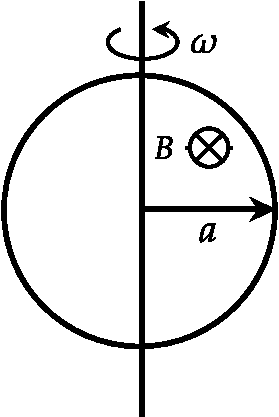
\includegraphics[height=4cm,width=2.8cm]{ED-20}
	\end{figure}
\item Self inductance per unit length of a long solenoid of radius $R$ with $n$ turns per unit length is:
	{\exyear{ JEST-2016}}
 \begin{tasks}(2)
	\task[\textbf{a.}]$\mu_{0} \pi R^{2} n^{2}$
	\task[\textbf{b.}]$2 \mu_{0} \pi R^{2} n$
	\task[\textbf{c.}]$2 \mu_{0} \pi R^{2} n^{2}$
	\task[\textbf{d.}] $\mu_{0} \pi R^{2} n$
\end{tasks}	
\item The $x-y$ plane is the boundary between free space and a magnetic material with relative permeability $\mu_{r}$. The magnetic field in the free space is $B_{x} \hat{i}+B_{z} \hat{k}$. The magnetic field in the magnetic material is
	{\exyear{ GATE- 2016}}
 \begin{tasks}(2)
	\task[\textbf{a.}]$B_{x} \hat{i}+B_{z} \hat{k}$
	\task[\textbf{b.}]$B_{x} \hat{i}+\mu_{r} B_{z} \hat{k}$
	\task[\textbf{c.}] $\frac{1}{\mu_{r}} B_{x} \hat{i}+B_{z} \hat{k}$
	\task[\textbf{d.}] $\mu_{r} B_{x} \hat{i}+B_{z} \hat{k}$
\end{tasks}	
\item 	At a surface current, which one of the magnetostatic boundary condition is $\underline{\text { NOT }}$ CORRECT?
{\exyear{ GATE- 2013}}
	 \begin{tasks}(2)
		\task[\textbf{a.}]Normal component of the magnetic field is continuous.
		\task[\textbf{b.}]Normal component of the magnetic vector potential is continuous.
		\task[\textbf{c.}] Tangential component of the magnetic vector potential is continuous.
		\task[\textbf{d.}] Tangential component of the magnetic vector potential is not continuous.
	\end{tasks}
\item A circular loop made of a thin wire has radius $2 \mathrm{~cm}$ and resistance $2 \Omega$. It is placed perpendicular to a uniform magnetic field of magnitude $\left|\vec{B}_{0}\right|=0.01$ Tesla. At time $t=0$ the field starts decaying as $\vec{B}=\vec{B}_{0} e^{-t / t_{0}}$, where $t_{0}=1 s$. The total charge that passes through a cross section of the wire during the decay is $Q$. The value of $Q$ in $\mu C$ (rounded off to two decimal places) is
{\exyear{ GATE- 2019}}
\item A long solenoid is embedded in a conducting medium and is insulated from the medium. If the current through the solenoid is increased at a constant rate, the induced current in the medium as a function of the radial distance $r$ from the axis of the solenoid is proportional to
{\exyear{GATE- 2015}}
 \begin{tasks}(2)
	\task[\textbf{a.}] $r^{2}$ inside the solenoid and $\frac{1}{r}$ outside
	\task[\textbf{b.}]$r$ inside the solenoid and $\frac{1}{r^{2}}$ outside
	\task[\textbf{c.}]$r^{2}$ inside the solenoid and $\frac{1}{r^{2}}$ outside
	\task[\textbf{d.}] $r$ inside the solenoid and $\frac{1}{r}$ outside
\end{tasks}
\item Consider an infinitely long solenoid with $N$ turns per unit length, radius $R$ and carrying a current $I(t)=\alpha \cos \omega t$, where $\alpha$ is a constant and $\omega$ is the angular frequency. The magnitude of electric field at the surface of the solenoid is
 \begin{tasks}(2)
	\task[\textbf{a.}]$\frac{1}{2} \mu_{0} N R \omega \alpha \sin \omega t$
	\task[\textbf{b.}]$\frac{1}{2} \mu_{0} \omega N R \cos \omega t$
	\task[\textbf{c.}]$\mu_{0} N R \omega \alpha \sin \omega t$
	\task[\textbf{d.}] $\mu_{0} \omega N R \cos \omega t$
\end{tasks}
\item A medium $\left(\varepsilon_{r}>1, \mu_{r}=1, \sigma>0\right)$ is semi-transparent to an electromagnetic wave when
{\exyear{ GATE- 2020}}
 \begin{tasks}(2)
	\task[\textbf{a.}]Conduction current $\gg>$ Displacement current
	\task[\textbf{b.}]Conduction current $<<$ Displacement current
	\task[\textbf{c.}]Conduction current $=$ Displacement current
	\task[\textbf{d.}] Both Conduction current and Displacement current are zero
\end{tasks}
\item A sinusoidal voltage of the form $V(t)=V_{0} \cos (\omega t)$ is applied across a parallel plate capacitor placed in vacuum. Ignoring the edge effects, the induced emf within the region between the capacitor plates can be expressed as a power series in $\omega$. The lowest nonvanishing exponent in $\omega$ is -----------
{\exyear{ GATE- 2020}}











\newpage
\begin{abox}
	Practise Set-3
\end{abox}
\begin{enumerate}
	\item 	The $x$ and $z$-components of a static magnetic field in a region are $B_{x}=B_{0}\left(x^{2}-y^{2}\right)$ and $B_{z}=0$, respectively. Find one of the possible solution for its $y$-component which is consistent with the Maxwell equations?
	\begin{answer}
		\begin{align*}
		 B_{x}&=B_{0}\left(x^{2}-y^{2}\right), B_{z}=0\\
		\because \vec{\nabla} \cdot \vec{B}&=0 \Rightarrow \frac{\partial B_{x}}{\partial x}+\frac{\partial B_{y}}{\partial y}+\frac{\partial B_{z}}{\partial z}=0 \Rightarrow \frac{\partial B_{y}}{\partial y}\\&=-\frac{\partial B_{x}}{\partial x}=-2 B_{0} x \Rightarrow B_{y}=-2 B_{0} x y
		\end{align*}
	\end{answer}
	\item 	Which of the following expressions represent an electric field due to a time varying magnetic field?
	\begin{tasks}(2)
		\task[\textbf{a.}]$K(x \hat{x}+\hat{y} \hat{y}+z \hat{z})$
		\task[\textbf{b.}]$K(x \hat{x}+y \hat{y}-z \hat{z})$
		\task[\textbf{c.}] $K(x \hat{x}-y \hat{y})$
		\task[\textbf{d.}] $K(y \hat{y}-x \hat{y}+2 z \hat{z})$
	\end{tasks}
\begin{answer}
	\begin{align*}
	\text { For time varying fields } &\vec{\nabla} \times \vec{E} \neq 0\\
	\text { (a) } \vec{\nabla} \times \vec{E}=K\left|\begin{array}{ccc}
	\hat{x} & \hat{y} & \hat{z} \\
	x & \partial / \partial y & \partial / \partial z \\
	y & z
	\end{array}\right|&=\hat{x}\left(\frac{\partial z}{\partial y}-\frac{\partial y}{\partial z}\right)+\hat{y}\left(\frac{\partial x}{\partial z}-\frac{\partial z}{\partial x}\right)+\hat{z}\left(\frac{\partial y}{\partial x}-\frac{\partial x}{\partial y}\right)=0\\
	\text { (b) } \vec{\nabla} \times \vec{E}=K\left|\begin{array}{ccc}
	\hat{x} & \hat{y} & \hat{z} \\
	\partial / \partial x & \partial / \partial y & \partial / \partial z \\
	x & y & -z
	\end{array}\right|&=\hat{x}\left(-\frac{\partial z}{\partial y}-\frac{\partial y}{\partial z}\right)+\hat{y}\left(\frac{\partial x}{\partial z}+\frac{\partial z}{\partial x}\right)+\hat{z}\left(\frac{\partial y}{\partial x}-\frac{\partial x}{\partial y}\right)=0\\
	\text { (c) } \vec{\nabla} \times \vec{E}=K\left|\begin{array}{ccc}
	\hat{x} & \hat{y} & \hat{z} \\
	\partial / \partial x & \partial / \partial y & \partial / \partial z \\
	x & -y & 0
	\end{array}\right|&=\hat{x}\left(0+\frac{\partial y}{\partial z}\right)+\hat{y}\left(\frac{\partial x}{\partial z}-0\right)+\hat{z}\left(-\frac{\partial y}{\partial x}-\frac{\partial x}{\partial y}\right)=0\\
	\text { (d) } \vec{\nabla} \times \vec{E}=K\left|\begin{array}{ccc}
	\hat{x} & \hat{y} & \hat{z} \\
	\partial / \partial x & \partial / \partial y & \partial / \partial z \\
	y & -x & 2 z
	\end{array}\right|&=\hat{x}\left(\frac{\partial(2 z)}{\partial y}+\frac{\partial x}{\partial z}\right)+\hat{y}\left(-\frac{\partial x}{\partial z}-\frac{\partial(2 z)}{\partial x}\right)+\hat{z}\left(\frac{\partial y}{\partial x}-\frac{\partial y}{\partial y}\right)\\
	\Rightarrow \vec{\nabla} \times \vec{E}&=-\hat{z} \neq 0
	\end{align*}
\end{answer}
	\item A uniform magnetic field in the positive $z$-direction passes through a circular wire loop of radius $1 \mathrm{~cm}$ and resistance $3.14 \Omega$ lying in the $x y$-plane. The field strength is reduced from 10 tesla to 9 tesla in $1 s$. Find the charge transferred across any point in the wire. 
	\begin{answer}
		\begin{align*}
		\varepsilon&=-\frac{d \phi}{d t} \Rightarrow I=\frac{d q}{d t}=\frac{\varepsilon}{R}=-\frac{1}{R} \frac{d \phi}{d t}\\
		\Rightarrow d q&=-\frac{A}{R} d B=\frac{-\pi r^{2}}{R} d B\\
		\Rightarrow d q&=\frac{-3.14 \times\left(10^{-2}\right)^{2}}{3.14} \times 1=10^{-4} \text { coulomb }
		\end{align*}
	\end{answer}
	\item A small loop of wire of area $A=0.01 \mathrm{~m}^{2}, N=40$ turns and resistance $R=10 \Omega$ is initially kept in a uniform magnetic field $B$ in such a way that the field is normal to the loop. When it is pulled out of the magnetic field, a total charge of $Q=2 \times 10^{-5} C$ flows through the coil. Find the magnitude of the field $B$.
	\begin{answer}
		\begin{align*}
		\text { Magnetic flux through the loop }& \phi=N B A\\
		\text { Induced e.m.f } \varepsilon&=-\frac{d \phi}{d t} \text { and induced current } i\\&=-\frac{1}{R} \frac{d \phi}{d t}=\frac{d Q}{d t} \Rightarrow-\frac{1}{R} d \phi=d Q \text {. }\\
		\text { Thus } \frac{1}{10} \times(40 \times B \times 0.01)&=2 \times 10^{-5} \Rightarrow B=5 \times 10^{-4} T
		\end{align*}
	\end{answer}
	\item A rectangular loop of dimension $L$ and width $w$ moves with a constant velocity $v$ away from an infinitely long straight wire carrying a current $I$ in the plane of the loop as shown in the figure below. Let $R$ be the resistance of the loop. Show that the current in the Toop at the instant the near side is at a distance $r$ from the wire is $\frac{\mu_{0} I L}{2 \pi R} \frac{w v}{r[r+w]}$.
	\begin{figure}[H]
		\centering
		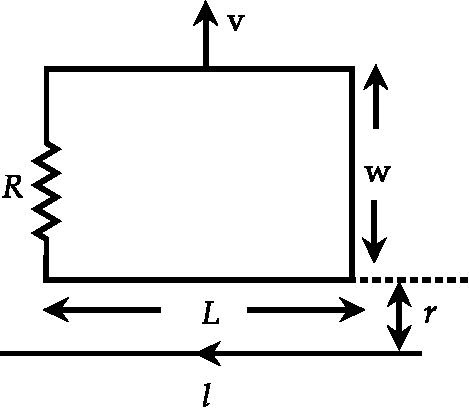
\includegraphics[height=3.5cm,width=4cm]{Ass-05}
	\end{figure}
\begin{answer}
	\begin{align*}
	\phi_{B}&=\int_{S} \vec{B} \cdot d \vec{a}=\int_{r}^{w} \frac{\mu_{0} I}{2 \pi r} L d r=\frac{\mu_{0} I L}{2 \pi R} \ln \left(\frac{r+w}{r}\right)\\
	\Rightarrow I&=-\frac{1}{R} \frac{d \phi_{B}}{d t}=\frac{\mu_{0} I L}{2 \pi R}\left[\frac{1}{r+w}-\frac{1}{r}\right] \frac{d r}{d t}=\frac{\mu_{0} I L w v}{2 \pi R r(r+w)}
	\end{align*}
\end{answer}
	\item A square loop of side $L$ and mass $M$ is made of a wire of cross-sectional area $A$ and resistance $R$ The loop. moving with a constant velocity $v_{v} \hat{i}$ in the horizontal xy-plane, enters a region $0 \leq x \leq 2 L$ having constant magnetic field $B \hat{k}$
	\begin{figure}[H]
		\centering
		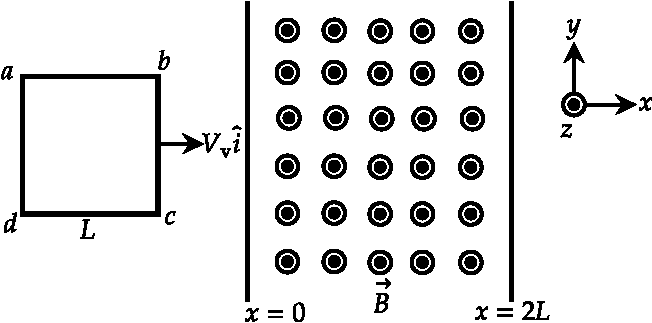
\includegraphics[height=4cm,width=8cm]{Ass-01}
	\end{figure}
	Find an expression for the $x$-component of the force $\vec{F}$ acting on the loop in terms of its velocity $\vec{v}(t), B, L$ and $R$.
	\begin{answer}
		\begin{align*}
		\text { Initial flux } \phi_{0}&=B L x\\
		\text { Flux after time } d t, \phi&=B L(x+d x)\\
		\text { Change in flux } d \phi&=\phi-\phi_{0}=B L d x \text {. }\\
		\text { Induced e.m.f. } \varepsilon&=-\frac{d \phi}{d t}=-B L \frac{d x}{d t}=-B L v_{0} \text {. }\\
		\text { Induced current } I_{i n d}&=-\frac{B L v_{0}}{R} \text { (in clockwise direction } a b c d a \text { ) }\\
		\text { Force on element } b c \vec{F}&=I_{\text {ind }} \int(d \vec{l} \times \vec{B})=-\frac{B^{2} L^{2} v_{0}}{R} \hat{x}
		\end{align*}
	\end{answer}
	\item A coil of 15 turns, each of radius 1 centimeter, is rotating at a constant angular velocity $\omega=300$ radians per second in a uniform magnetic field of $0.5$ tesla, as shown in the figure. Assume at time $t=0$ that the normal $\hat{n}$ to the coil plane is along the $y$-direction and that the self-inductance of the coil can be neglected. If the coil resistance is 9 ohms, what will be the magnitude of the induced current in milliamperes?
	\begin{figure}[H]
		\centering
		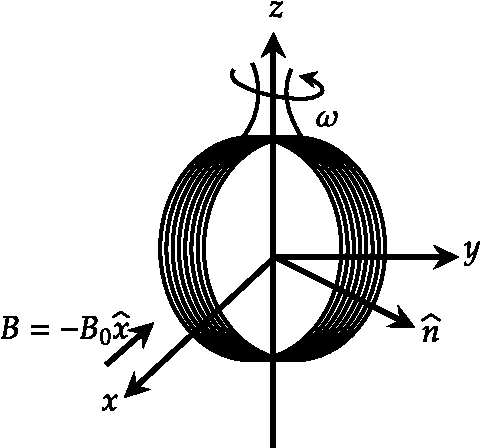
\includegraphics[height=3.8cm,width=4.3cm]{Ass-02}
	\end{figure}
\begin{answer}
	The voltage induced is equal to the change in magnetic flux
	\begin{align*}
	\varepsilon=-\frac{\partial \Phi}{\partial t}, \text { where } \Phi=\int \vec{B} \cdot d \vec{A}
	\intertext{Noting the initial condition $(\Phi(t=0)=0)$, since the field and area normal are perpendicular). One finds that $\Phi=\int \vec{B} \cdot d \vec{A}=B \cos (90+\omega t) \pi r^{2}=(-B \sin \omega t) \pi r^{2}$.
		Thus, $|d \Phi / d t|=\omega B \cos (\omega t) \pi r^{2}$.}
	\intertext{Now, to find the current, one uses Ohm's Law in Faraday's Law to get}
	I=\frac{N \dot{\Phi}}{R}&=\frac{N B \omega}{R} \cos (\omega t) \pi r^{2} \text {, where } N \text { is the number of turns. }\\
	\text { Thus, } I=\frac{15 \times 0.5 \times 300}{9} \cos (\omega t) \pi(1 / 100)^{2}&=250 \times 10^{-4} \pi \cos (\omega t) \text { Ampere }I=25 \pi \cos (\omega t) \mathrm{mA}
	\end{align*}
\end{answer}
	\item The circuit shown below is in a uniform magnetic lield that is into the page and is decreasing in magnitude at the rate of 150 Tesla/sec. Then tind the ammeter reading.
	\begin{figure}[H]
		\centering
		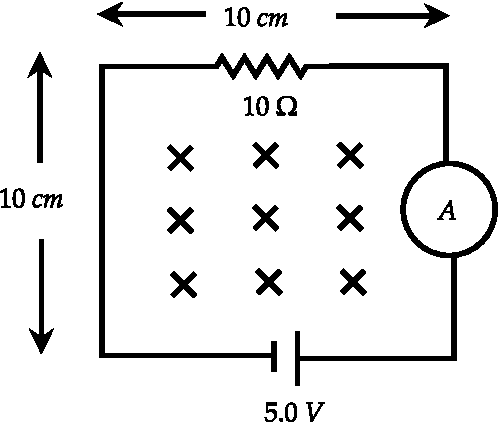
\includegraphics[height=4.5cm,width=5cm]{Ass-03}
	\end{figure}
\begin{answer}
 From Ohm's Law $V-\varepsilon=I R$, one can obtain the current. (Note that $V=5.0 \mathrm{~V}$ is the voltage of the battery. The voltage induced acts to oppose this emf from the battery).
	\begin{align*}
	\text { The problem gives } \frac{d B}{d t}&=150 T / \mathrm{s} \text {. The area is just } 0.01 \mathrm{~m}^{2} \text {. }\\
	\text { Thus, the induced emf is, } \varepsilon&=\frac{d B}{d t} \quad A=150 \times 0.01=1.5\\
	\text { Thus, } V-\varepsilon&=3.5=I R \Rightarrow I=0.35 A \text {, since } R=10 \Omega \text {. }
	\end{align*}
\end{answer}
	\item A parallel plate air-gap capacitor is made up of two plates of area $10 \mathrm{~cm}^{2}$ each kept at a distance of $0.88 \mathrm{~mm}$. A sine wave of amplitude $10 \mathrm{~V}$ and frequency $50 \mathrm{~Hz}$ is applied across the capacitor as shown in the figure.
	\begin{tasks}(1)
		\task[\textbf{a.}]Find the amplitude of the displacement current density between the plates.
		\task[\textbf{b.}]
		 Find the r.m.s value of the displacement current density between the plates.
		\task[\textbf{c.}]Find the average value of the displacement current density (in $\mathrm{mA} / \mathrm{m}^{2}$ ) between the plates.
	\end{tasks}
	\begin{figure}[H]
		\centering
		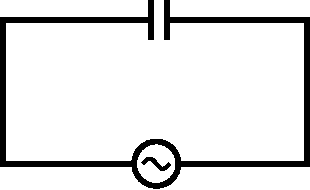
\includegraphics[height=2.5cm,width=4cm]{Ass-04}
	\end{figure}
\begin{answer}
	\begin{align*}
	\text { Displacement current density } J_{d}&=\varepsilon_{0} \frac{\partial E}{\partial t}=\frac{\varepsilon_{0}}{d} \frac{\partial V(t)}{\partial t}=-\frac{\varepsilon_{0} \omega V_{0} \sin \omega t}{d}\\
	\text { (a) Amplitude of the displacement current density } J_{0 d}&=\frac{\varepsilon_{0} \omega V_{0}}{d}=\frac{2 \pi \varepsilon_{0} f V_{0}}{d}\\
	\Rightarrow J_{0 d}=4 \pi \varepsilon_{0} \frac{f V_{0}}{2 d}&=\frac{1}{9 \times 10^{9}} \frac{50 \times 10}{2 \times 88 \times 10^{-5}}=0.03 \mathrm{~mA} / \mathrm{m}^{2}
	\intertext{(b) The r.m.s value of the displacement current density is }
	J_{d, r m s}=\frac{\varepsilon_{0} \omega V_{0}}{d \sqrt{2}}=\frac{2 \pi \varepsilon_{0} f V_{0}}{d \sqrt{2}}&=\frac{0.03}{\sqrt{2}}=0.022 \mathrm{~mA} / \mathrm{m}^{2}
	\intertext{(c) The average value of the displacement current density is zero. }
	\end{align*}
\end{answer}
\end{enumerate}

















	
	
	
	
	
	
	
	
	
	
\end{enumerate}




\newpage
\begin{abox}
	Practise Set-4
\end{abox}
\begin{enumerate}
	\item 	The $x$ - and $z$-components of a static magnetic field in a region are $B_{x}=B_{0}\left(x^{2}-y^{2} x\right)$ and $B_{z}=0$, respectively. Which of the following solutions for its $y$-component is consistent with the Maxwell equations?
	 \begin{tasks}(2)
		\task[\textbf{a.}]$B,=B_{0} x y$
		\task[\textbf{b.}]$B_{y}=-2 B_{0} x y$
		\task[\textbf{c.}]$B_{y}=-B_{0}\left(x^{2}-y^{2}\right)$
		\task[\textbf{d.}] $B_{y}=-B_{0}\left(2 x y-\frac{1}{3} y^{3}\right)$
	\end{tasks}
\item 	Let the electric field in some region $R$ be given by $\bar{E}=e^{-y^{2}} \hat{i}+e^{-x^{2}} \hat{j}$. From this we may conclude that
	 \begin{tasks}(1)
		\task[\textbf{a.}]$R$ has a non-uniform charge distribution
		\task[\textbf{b.}] $R$ has no charge distribution
		\task[\textbf{c.}]$R$ has a time independent magnetic field
		\task[\textbf{d.}]  The energy flux in $R$ is zero everywhere
	\end{tasks}
\item A parallel plate capacitor has circular plates of radius $R$. It is being charged by a current $I$. Then the magnetic induction $\vec{B}$ at a point between the plates at a distance $R / 2$ from the axis of the capacitor is:
	 \begin{tasks}(2)
		\task[\textbf{a.}]$\vec{B}=\frac{\mu_{0} I}{2 \pi R} \vec{\phi}$
		\task[\textbf{b.}]$\vec{B}=\frac{\mu_{0} I}{4 \pi R} \hat{\phi}$
		\task[\textbf{c.}]$\vec{B}=\frac{\mu_{0} l}{6 \pi R} \hat{\phi}$
		\task[\textbf{d.}]  $\vec{B}=\frac{\mu_{0} J}{8 \pi R} \hat{\phi}$	
	\end{tasks}
\item 	The divergence of a magnetic field $\vec{B}(\vec{r}, t)$ from a time varying current density $\vec{J}(\vec{r}, t)$ is
	 \begin{tasks}(1)
		\task[\textbf{a.}]always zero as there are no magnetic monopoles
		\task[\textbf{b.}] non-zero and proportional to the rate of change of electric field $\vec{E}(\vec{r}, t)$ from the current density
		\task[\textbf{c.}]non-zero and proportional to the divergence of electric field $\vec{E}(\vec{r}, t)$ from the current density
		\task[\textbf{d.}]  non-zero and proportional to the current density
	\end{tasks}
\item A charged capacitor $(C)$ is connected in series with an inductor $(L)$. When the displacement current reduces to zero, the energy of the $L C$ circuit is
	 \begin{tasks}(1)
		\task[\textbf{a.}]stored entirely in its magnetic field.
		\task[\textbf{b.}] stored entirely in its electric field.
		\task[\textbf{c.}]distributed equally among its electric and magnetic fields.
		\task[\textbf{d.}]  radiated out of the circuit.
	\end{tasks}
\item 	Maxwell's equations can be writton in the form shown below. If magnetic charge exists and if it is conserved, which of these equations will have to be changed?\\
I. $\nabla \cdot E=\rho / \varepsilon_{0}$\\
Il. $\nabla \cdot \mathrm{B}=0$\\
III. $\nabla \times \mathrm{E}=-\frac{\partial \mathrm{B}}{\partial t}$\\
IV. $\nabla \times \mathrm{B}=\mu_{0} J+\mu_{0} \varepsilon_{0} \frac{\partial \mathrm{E}}{\partial t}$
	 \begin{tasks}(2)
		\task[\textbf{a.}] Ionly
		\task[\textbf{b.}]Il only
		\task[\textbf{c.}]III only.
		\task[\textbf{d.}]II and III 
	\end{tasks}
\item One of Maxwell's equations is $\vec{\nabla} \cdot \overrightarrow{\mathrm{B}}=0$. Which of the following sketches shows magnetic field lines that clearly violate this equation within the region bounded by the dashed lines?	 
  \begin{tasks}(2)
 	\task[\textbf{a.}]
 	\begin{figure}[H]
 		\centering
 		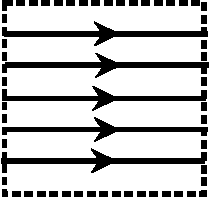
\includegraphics[height=2.5cm,width=2.5cm]{Ass-06}
 	\end{figure}
 	\task[\textbf{b.}]	\begin{figure}[H]
 		\centering
 		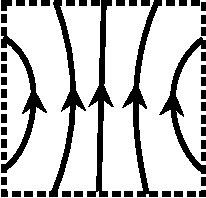
\includegraphics[height=2.5cm,width=2.5cm]{Ass-07}
 	\end{figure}
 	\task[\textbf{c.}]	\begin{figure}[H]
 		\centering
 		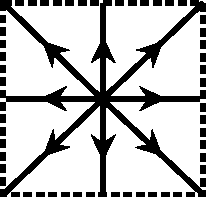
\includegraphics[height=2.5cm,width=2.5cm]{Ass-08}
 	\end{figure}
 	\task[\textbf{d.}] 	\begin{figure}[H]
 		\centering
 		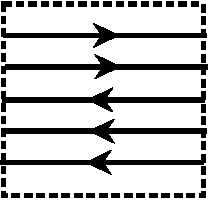
\includegraphics[height=2.5cm,width=2.5cm]{Ass-09}
 	\end{figure}
 \end{tasks}
	
	
	
	
	
	
	
	
	
	
	
	
	
	
	
	
	
	
	
	
\end{enumerate}










































